\documentclass[11pt]{article}
\usepackage{deauthor,times,graphicx}
\usepackage{url}
\usepackage{hyperref}
\renewcommand{\UrlFont}{\fontfamily{cmvtt}\selectfont}
\usepackage{wrapfig}

\usepackage[font=small,labelfont=bf]{caption}

% Create small items.
\newcommand{\smallitem}[1]{\vspace{0.3em}\noindent\textbf{#1}}
\newcommand{\smallitembot}{\vspace{0.5em}\noindent}

% Note-related commands.
\usepackage{etoolbox}
\usepackage{xcolor}
\newcommand{\jmh}[1]{\textcolor{blue}{jmh: #1}}
\newcommand{\jeff}[1]{\textcolor{green}{jeff: #1}}
\newcommand{\sean}[1]{\textcolor{purple}{sean: #1}}

\title{Self-Service Data Preparation: Research to Practice}
\author{Joseph M. Hellerstein, Jeffrey Heer and Sean Kandel\\
{\small \{joe, jheer, skandel\}@trifacta.com}}
\date{May 2018}

\begin{document}

\maketitle

\section{The Arrival of the Category}
It is widely accepted that the majority of time in any data analysis project is devoted to preparing the data~\cite{nyt-janitor}. In 2012, noted data science leader DJ Patil put the fraction of time spent on data preparation at 80\%, based on informal discussions in his team at LinkedIn~\cite{patil2012data}. Analysts we interviewed in an academic study around the same time put the percent time ``munging'' or ``wrangling'' data at ``greater than half''~\cite{interviews}. Judging from these user stories, the inefficiency of data preparation is the single biggest problem in data analytics.

The database community does have a tradition of research on related topics. Most common is algorithmic work (covered in various surveys, e.g.~\cite{ilyas2015trends,doan2012principles,chu2016data, marcus2015crowdsourced}) that focuses on automating certain aspects of data integration and cleaning, or that uses humans as passive computational elements via crowdsourcing. 

What computer science researchers often miss are the skills realities in real-world organizations. In practice, the primary bottleneck is not the quality of the inner-loop algorithms, but rather the lack of technology enabling domain experts to perform end-to-end data preparation without programming experience. Fully preparing a dataset requires an iterated cycle of input data quality assessment, transform specification, and output quality assessment---all in service of a larger ``preparedness'' goal that tends to shift fluidly as the work reveals additional properties of the data. Traditionally there has been a divide between the people who know the data and use case best, and the people who have the skills to prepare data using traditional programmatic approaches. This results in the data preparation cycle being split across parties and across time: domain experts try to express their desired outcomes for prepared data to developers or IT professionals, who in turn try to satisfy the needs. A single iteration of this cycle can take from hours to weeks in a typical organization, and rarely produces a satisfying outcome: typically either the end-user did not specify their desires well, or the developer did not achieve the desired outcome. Neither tends to enjoy the experience. In short, the primary problem in data preparation is \emph{self-service}: we need to enable the people who know the data best to prepare it themselves.

Research focused on these user-facing concerns is scattered across the fields of databases, HCI and programming languages (e.g., ~\cite{galhardas2000ajax,raman2001potter,hernandez2001clio,mandelbaum2007pads,kandel2011wrangler,gulwani2011automating,jin2017foofah}). While under-investigated in the research community, the topic has become an important force in the industry. In 2015, industry analysts began publishing rankings in an emerging new market category dubbed ``Self-Service'' or ``End-User'' Data Preparation~\cite{dresner, bloor}. Two years later, the established analyst firm Forrester did a first annual Forrester Wave report on Data Preparation~\cite{forrester-wave}: a mark of arrival for this category. Another major analyst firm, Gartner, has weighed in with various reports on the Data Preparation market (e.g.~\cite{gartner-marketguide-2017, gartner-peer-insights}). Meanwhile, in 2017 Google Cloud Platform was the first cloud provider to launch Self-Service Data Preparation as a native service in their cloud~\cite{novet-dataprep}, while Azure and Amazon Web Services also announced partnerships with data preparation vendors in 2018.  Market size estimates for Data Preparation start at \$1 billion~\cite{gartner-marketguide-2017} and go well upwards depending on the analyst and projected time horizon. Not bad for a technology that was seeded from academic research, and did not even have a name four years ago.

\pagebreak
In this article we share some of our experience navigating the path from research to commercial products in this domain, which we and our users at Trifacta affectionately refer to as Data Wrangling. 
We begin by providing a snapshot of the space as we are seeing it, including motivating customer use cases, and distinctions between the new Data Wrangling market and co-existing older markets in Data Integration and ETL. Then we go back to the research roots of Trifacta and talk about how our views of users and technical requirements have evolved.

\subsection{A Data Wrangling Case Study}
\label{sec:casestudy}
At Trifacta, we have seen Data Wrangling use cases in a wide variety of contexts and markets; any organization that does data analysis needs to do data preparation. There is broad usage in traditional industries like financial services, telecommunications, pharmaceuticals and health care. But we also see interesting use cases in everything from assembling national voter rolls for the 2016 presidential election % ~\cite{nationbuilder} 
to decoding data from drones. %~\cite{flyspan}.


As a case study, consider the following example usage in public health. In late 2014 there was surge of HIV cases in rural Scott County, Indiana, which eventually infected nearly 200 people. The US Center for Disease Control (CDC) came in to study patients and assemble a large number of data sources, and found that sharing of opioid needles was the primary vector for infection. Their recommendation for the best way to stop the spread of AIDS in Scott County: establish clean needle exchanges for drug users.  The governor of Indiana at the time, Mike Pence, was ``morally opposed to needle exchanges on the grounds that they supported drug abuse''. However, after the CDC made its recommendation, the governor said ``I'm going to go home and pray on it''. In the end, Gov. Pence reportedly ``found the science convincing'', and approved the needle exchanges. This was 21 months before Pence became Vice President of the US.~\cite{nyt}.

During the investigation, the CDC worked under time pressure with a number of disparate data sets including ``HIV outbreak clusters, geographic factors, epidemiological patterns, and drug resistance data, among others''~\cite{datanami}. They brought in a systems integrator called Leidos who provided a software platform called CAADS that combines visual data technologies from multiple vendors: Trifacta for data preparation, Tableau for charting, and Alpine Data and Centrifuge Analytics for analytics. Leidos staff reported that Trifacta substantially reduced time for wrangling. ``Work that would have taken six weeks now can take as little as a day''~\cite{ravi}. CDC researchers also noted that Trifacta enabled them to detect missing records and outliers that would have otherwise polluted the analysis, and that were overlooked by prior data cleaning tools~\cite{leidos}.

The CDC is now recommending that state health departments prepare and monitor data from an increasingly large pool of sources on an ongoing basis, ``to identify jurisdictions that, like this county in Indiana, may be at risk of an IDU-related HIV outbreak.  These data include drug arrest records, overdose deaths, opioid sales and prescriptions, availability of insurance, emergency medical services, and social and demographic data''~\cite{cdc}.

Some of the key--and archetypal--features of this example include the following:

    \smallitem{Self Service:} The data was being acquired, prepared and analyzed not by computer experts, but by the domain experts who understood the data best: public health experts in the field. ``CAADS is very much built to ... support the range of public health aspects and to allow people who would otherwise not be able to get into data analytics to have access and do so in a responsible way.''~\cite{datanami} 
    
    \smallitem{Agility:} The users were engaged in rapid collaboration with visual tools to explore multiple hypotheses in a lightweight iterative fashion. ``They would be on a call discussing the outbreak and someone would say `What if we did it this way?' They'd step away for a minute, run the analysis, and say, `No that didn't work. But if we do it this other way, here's the result'''~\cite{datanami}.
    
    \smallitem{Veracity and Explainability:} The results of the study were to be presented for executive decision-making with an expectation of critical feedback. In that setting, intuitive explanations of recommendations were critical.
    
    \smallitem{More Data, More Data Sources:} The Indiana effort involved a wide range of data, acquired quickly from a variety of source in a variety of ways. Looking ahead, the CDC expects this set of sources to grow, and sees a need to monitor feeds from these sources over time.
\smallitembot

\section{Key Tasks in Data Wrangling}
Here we briefly overview the main tasks in wrangling data. For a more thorough treatment we refer the reader to a book on the subject~\cite{rattenbury2015data}.

\smallitem{Unboxing: Discovery \& Assessment}: If you have worked with new data you know that the first step is the wonder of unboxing: what's in there? Basic questions arise right away. How is the data structured: does it have discrete records and fields? Is it flat or nested, uniform or irregular, dense or sparse? Is there metadata embedded in the data that should be pulled out? What types of fields are there, and how are they coded? Do particular values of interest occur in the data...am I in the data? What are the data distributions: the popular and rare categorical variables, the distribution of numerical variables?   You cannot begin thinking about data analysis before understanding the answers to these basic questions. Visualization can help a great deal here, but note that only the last questions above match typical charting packages and BI. The other questions relate more closely to parsing and second-order schematic transformations that involve manipulating both data and metadata.

\smallitem{Structuring}. Analytics software likes its data in rectangles: tables or matrices. Different rectangles fuel different analyses: sometimes a matrix or pivot table is the right thing, other times a relational table is better.  As a result, it is common to restructure data whether or not it arrives structured. Typical (re)structuring transformations include pivoting tables into matrices and vice versa, as well as unnesting key/value sets (``dictionaries'', ``maps'' or ``objects'') or arrays/lists into columns. These transforms have the property that they convert data (say keys in a JSON document) into metadata (column names) or vice versa: they are second order data transformations unfamiliar from SQL and logic. Users tend to find these transformations very non-intuitive, so various visual metaphors are often used to help users route values to appropriate coordinates in a grid.

\smallitem{Cleaning}. Neat is not the same as clean: tabular or matrix data can often be dirty in the sense of failing to capture expectations. One class of expectations capture the notion of ``central'' and ``outlying'' values. Outliers can be statistical (e.g. distance from the center of a distribution) or semantic ('Italy' is the not the name of a US state.) Another class of expectations are logical: boolean properties like functional dependencies. Yet another class relates to encoding: e.g., in entity resolution, objects with multiple categorical labels need to have their labels mapped together. Expectation checking for data cleaning often involves consideration of individual records with respect to a larger dataset or population, which can be difficult for humans to do manually---algorithms are needed. But the outputs of these algorithms are often uncertain or ambiguous, and human intervention can be required to complete the job. The surveys mentioned earlier provide overviews of these issues~\cite{ilyas2015trends,doan2012principles,chu2016data,marcus2015crowdsourced}, but some of the hardest problems are in enabling users to assess and correct algorithm outputs.

\smallitem{Enriching \& Blending}. Data is rarely self-contained; it often benefits from or requires additional data for further context. As a simple example, unresolved ``reference'' or ``foreign key'' identifiers need to be decoded by joining to a lookup table. Softer issues also drive the need for data enrichment: for example, to assess the likelihood of the data you have, you may want to compare it to a larger sample from a similar or different population. Or to assess the significance of a correlation between two attributes in your data (say, disease occurrence and age) you may want to join in a third column from another data set to establish if there is conditional independence via a confounding variable (say tobacco use). Algebraically, these activities---often called ``data blending'' in industry marketing material---encompass a range of transformations including joins, unions, and subqueries with aggregation. It is not always easy to figure out how to do these tasks, or to assess if they were done correctly.

\smallitem{Optimizing \& Publishing}. Once a dataset is structured and cleaned to an analyst's level of comfort, it is often necessary to do additional preparation to produce appropriate output for the next phase of analysis. For example, publishing data to a relational data warehouse may require normalizing a single nested dataset into a number of tables with key/foreign key relationships. The traditional schema mapping problem that occupied the ETL and Data Integration communities during the 1990's can be viewed as a general example of this kind of work. In modern ``big data'' environments with machine-generated data, it is often necessary to perform data reduction before visualizing the results in a traditional charting tool: aggregation or sampling of the cleaned data is still required. In other cases, data has to be recoded to suit the specific API of a downstream product for analysis or charting. These tasks can be as demanding and detail-oriented as any of the other steps in the pipeline. 
\smallitembot{}

In sum, in 2018 we should all be aware that data is not ``truth'': it is evidence to be assessed in the context of specific use cases. If your data is familiar, your use case may change---or vice versa---requiring you to rethink some or all of the steps above. 

% While the tasks above are presented as discrete and isolated, they in fact overlap quite a bit. For example, assessment is endemic in almost every step, and it changes relative to the task whose output is being assessed. Blending and Structuring are sometimes the same, sometimes duals (e.g. during normalization you may ``unblend'' joinedip data). And so on. It is also the case that the overall process of data preparation does not march through these tasks in any linear fashion. In short, data preparation is an iterative and subjective process that requires human ``taste'' and domain expertise. The above gives a flavor of the typical tasks, but is neither comprehensive nor a perfect breakdown.

% \subsection{Using Trifacta}~\label{sec:lifecycle}
% The lifecycle of a data transformation job in Trifacta works roughly as follows.  First, the user creates a ``Flow'': a project to work with one or more datasets. Then, they add datasets to the flow. Datasets are not stored in Trifacta, they are registered by reference to any of a variety of sources including hosted filesystems and database systems either on premises or in the cloud. (Desktop files can be uploaded through Trifacta to a hosted filesystem for processing.) Then the user begins transforming datasets in the Trifacta Transformer interface, which allows both single-dataset and cross-dataset transformations. For modest-sized datasets, the user manipulates them directly in the Transformer; for large datasets, the user is given a sample to work on in the Transformer. User transformations are done visually and reflected immediately in the user interface, complete with visual profiling and data quality assessment at each step. When the user is satisfied with their flow, they can run a job to generate an output---this usage is common in single-use and exploratory environments. They can also schedule jobs to run on a regular basis, fetching data from the referenced sources and generating new output files---this usage is common in production environments. Outputs can be published in a variety of ways: to files, databases, visualization tool formats, and so on.

\subsection{Isn't this just ETL? Not really.}
At a high level, ETL and data preparation solve similar problems: transforming multiple input datasets to some desired output.  However, modern data preparation differs from ETL in nearly every basic question of Who, Why, What and Where, resulting in very different requirements for new software solutions.

ETL technologies are targeted at IT professionals (Who), tasked with establishing static data pipelines for reference data (Why), given structured inputs (What) in on-premises datacenters running legacy software (Where). These ETL systems
exist to help IT implement data pipelines for downstream consumers.  IT receives data requirements from a line of business, and implements and optimizes these pipelines on behalf of those consumers. IT is also responsible for ensuring security and quality of the data used by analysts.  The ``Who'' does not scale well with the rising tide of data: As organizations become more data-driven and the number of consumers and analytic use cases grows,  IT can become an unscalable bottleneck in the analysis lifecycle.

Data preparation tools instead focus on enabling analysts in a specific line of business (Who) to design and maintain data preparation recipes that solve problems relevant to the their job success (Why). They typically bring bespoke data from their own processes, and often blend in external data as well (What). In many cases these organizations are working on net new projects, and are given the latitude to set up on new modern infrastructure, e.g. using public clouds or open source technologies (Where).

The difference in the Who drives the need for self-service technology, reflecting the changing nature of data in large organizations. The line of business likes self-service data preparation because they best understand their own requirements, and self-service cuts out time-consuming communication and delivery cycles with IT. IT increasingly likes self-service, because analysts are not burdening them with tedious and ill-specified data provisioning requests.  Self-service data preparation enables organizations to scale the number of analysis tasks they can perform beyond what IT could centrally manage, and make the whole process more efficient and satisfying. Moreover, the change in Why often makes these exercises highly valuable: line-of-business use cases typically use data to  make more money or reduce costs. This is creative, competitive data work.

The difference in What is not to be minimized. Legacy ETL is designed to handle well-structured data
originating from a variety of operational systems or databases. Many ETL tools are entirely schema-driven: users are not shown data when they specify ETL pipelines. This makes it a poor fit to data that is not clearly schematized in one uniform way, or data that needs cleaning as much as it needs republishing. A growing amount of analysis occurs in environments where the schema of data is not defined or known ahead of time. This means the analyst doing the wrangling determines how the data can be leveraged for analysis as well as the schema (structure) to be imposed to perform that analysis.
Legacy ETL systems were not optimized for large-scale data or complex raw sources that require substantial restructuring and derivation.
 
Finally the Where is changing quickly. To be most effective, ETL and data preparation products should both be integrated into an ecosystem of other tools for storage, processing and consumption.  Legacy ETL products were designed when most data was on-premises in relational and operational systems.  Because the locus of data gravity is moving to big data and cloud environments, many forward-looking data preparation solutions are focused on working well in those environments.

This is not to say that ETL is dead. Like many legacy technologies, it plays a key role in the standard operating procedure of traditional IT. Rather, the point is that data preparation solutions should provide a new How to respond to the new Who, Why, What and Where. Legacy ETL use cases are already handled adequately, and there is less of a pressing need for new technologies to solve those old problems.



\section{Evolutionary Paths}
We launched the original Wrangler prototype on an academic website in Fall 2011, and quickly saw thousands of unique users: our first feedback on the importance of the area.
Since that time, we have been through many iterations of refining our understanding of the data wrangling problem and the key issues in improving user productivity. Here we share our learning on a number of fronts, from users to interfaces to backend systems.

\subsection{Personas}
A critical question for any product, but especially in an emerging market, is this: Who are my users? This question can be particularly difficult to answer in the early stages of design, when there are few if any actual users and instead one has to develop \emph{personas} of who the likely intended users are. Personas are ``fictional representations and generalizations of ... your target users who exhibit similar attitudes, goals, and behaviors in relation to your product.''~\cite{personas}. In the case of Trifacta, our understanding of who we are designing for has evolved tremendously as we have engaged different user communities and observed industry-wide changes in organizational data analysis roles.

Unsurprisingly, our initial outlook was anchored in the university environment in which we were pursuing research. We were motivated by our own trials and tribulations with data wrangling, as well as those of our academic peers. This orientation was reflected in our early user studies~\cite{wrangler, proactive-wrangler}: largely due to convenience, a majority of our study participants were computer science students with some degree of analysis training.

We recognized the limits of studying this population, and
set out
to conduct an interview study of analysts in industry~\cite{interviews}, involving professionals with varied titles such as ``business analyst'', ``data analyst'' and ``data scientist''. We found that our respondents were well-described by three archetypes (``hackers'', ``scripters'', and ``application users'') that differed in terms of skill set and typical workflows. These archetypes varied widely in terms of programming proficiency, reliance on information technology (IT) staff, and diversity of tasks, but varied less in terms of statistical proficiency. These initial archetypes, and their corresponding tasks and workflows, served as a major touchstone for our early commercialization efforts.

That is not, however, to say that our archetypes were unbiased. The analysts we interviewed at that time spanned a spectrum of programming proficiency, but all worked in dedicated analysis positions.  
Increasingly we see people working with data when that is not their primary job role: our case study in Section~\ref{sec:casestudy} is an example. In addition, we have observed industry-wide shifts in six years as ``data science'' has matured. While early data scientists were often a ``jack of all trades'' with a mix of skills including statistical analysis and large-scale processing, many organizations eventually differentiated the roles of data scientist (more focused on analytical tasks) and data engineer (more focused on analysis infrastructure). Moreover, traditional IT departments still play a critical role in organization-wide data efforts, but were not a focus of our interview study.

In the six years since our interviews, engagement with customers (including user studies, site visits, surveys, and interviews) has led us to refine and expand our personas. 
For example, while highly-skilled data scientists remain a constituency, we focus on them less than we did on campus. Users with programming ability often choose to complete data wrangling tasks using code, foregoing the efficiency and feedback afforded by improved visual tools in favor of the familiar walled garden of their favorite programming language. 
On the other hand, analysts in a specific line of business have driving questions and deep domain expertise, but may lack either the time or programming knowledge to write scalable data transformation code. These users also greatly outnumber data scientists, and so represent a larger business opportunity. 
Separately, we have learned to appreciate an additional class of user other than the data analyst:
users tasked with operationalizing, scheduling, and deploying workflows generated by self-service analysts. These users often need to oversee the use of computing resources, and the governance of data---an issue made all the more clear by the recent focus on privacy and the GDPR legislation in Europe. Some Trifacta customers choose the product not for its ease of use, but because it can be used to ensure a reliable, auditable process for preparing data for legislative or administrative compliance. 

\subsection{Interface Evolution}
\begin{wrapfigure}{R}{0.6\textwidth}
        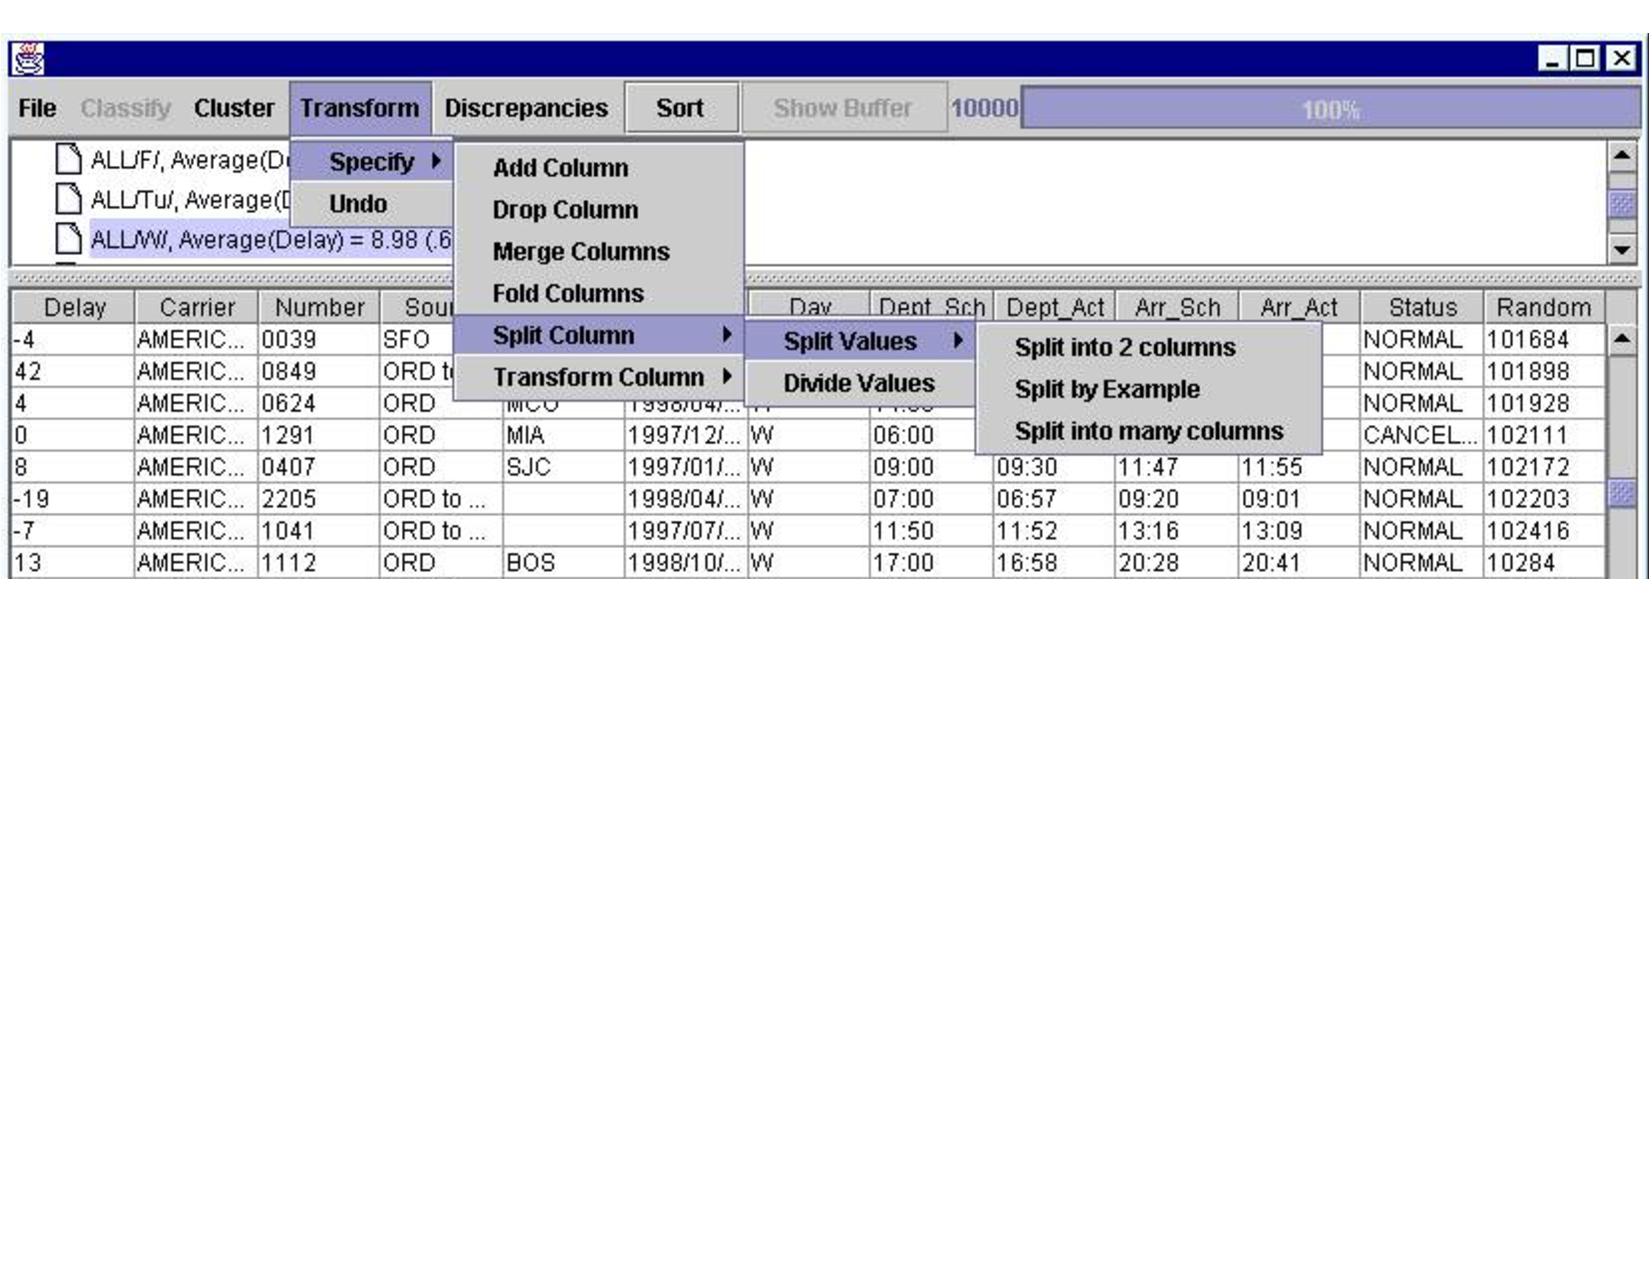
\includegraphics[width=0.6\textwidth]{figs/pwheel.pdf}
        \caption{Potter's Wheel with its menu-driven interface}
        \label{fig:pwheel}
\end{wrapfigure}
Data wrangling is fundamentally a programming task: users must choose a sequence of transformations to raw data, mapping it into a more usable and actionable form. Many data preparation solutions, including ours, formulate a \emph{domain-specific language (DSL)} for expressing the various transformations needed, such as formatting, filtering, aggregation, and integration operations. While writing high-level DSL programs can be an attractive alternative to writing low-level code in a more general language, it still imposes a technical burden. Instead, at Trifacta we enable end users to express DSL statements through interactions with a graphical user interface.

A primary source of inspiration was Raman \& Hellerstein's Potter's Wheel system~\cite{raman2001potter}. Potter's Wheel involved a scalable table grid view for directly inspecting data, coupled with menu-driven commands (and accompanying modal dialogs) for applying transformations (Figure~\ref{fig:pwheel}). These graphical commands were translated into statements in an underlying DSL: a sequence of user commands generates a data transformation script.

\begin{wrapfigure}{R}{0.6\textwidth}
        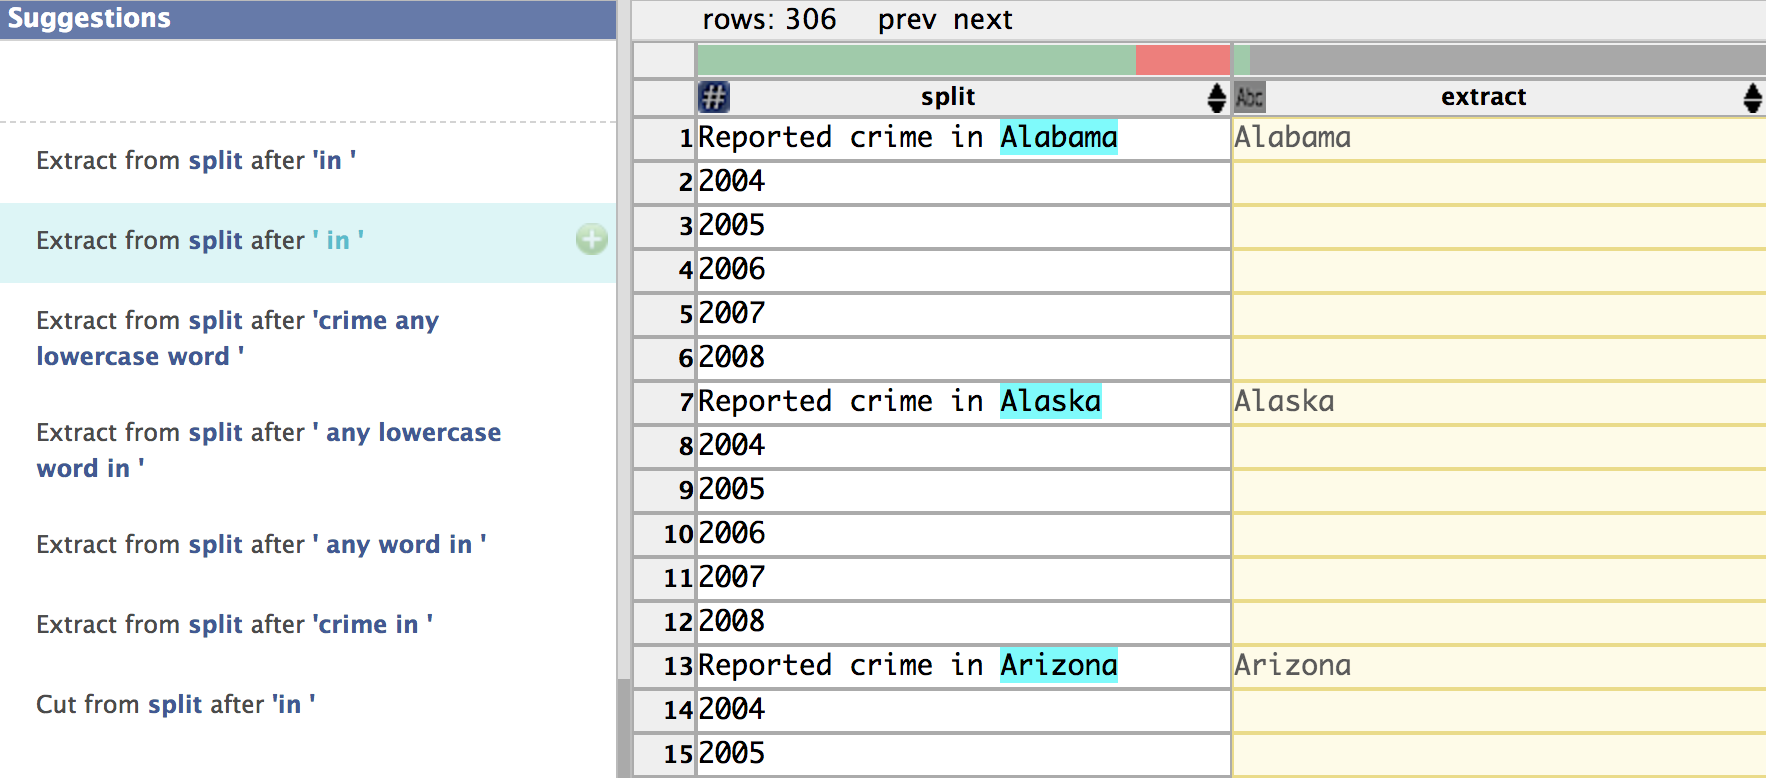
\includegraphics[width=0.6\textwidth]{figs/wrangler.png}
        \caption{Wrangler research prototype, with predictive interaction.}
          \label{fig:wrangler}
\end{wrapfigure}
In lieu of menus, our Data Wrangler research prototypes~\cite{wrangler, proactive-wrangler} focused on more direct manipulation interactions. We initially explored interface gestures for expressing transformations, but this led to ambiguity, as the same gesture might be used for different transformations. For example, if you select a span of text, do you intend to extract, replace, or split up the text? However, we realized that for a range of simple interactions (e.g., row, column, and text selection), typically only a small number of transformations make sense. This insight led us to an approach called \emph{predictive interaction}, analogous to auto-complete, in which simple gestures guide automated predictions of which transformations to apply. The system searches over relevant DSL statements compatible with the user selection and recommends those it believes will most improve the data~\cite{cidr-pi}. To help users select among the suggestions, we provided transformation summaries in a natural text format and visualizations that conveyed the effect the transformation would have on the data table (Figure~\ref{fig:wrangler}).


\begin{wrapfigure}{R}{0.4\textwidth}
    \centering
    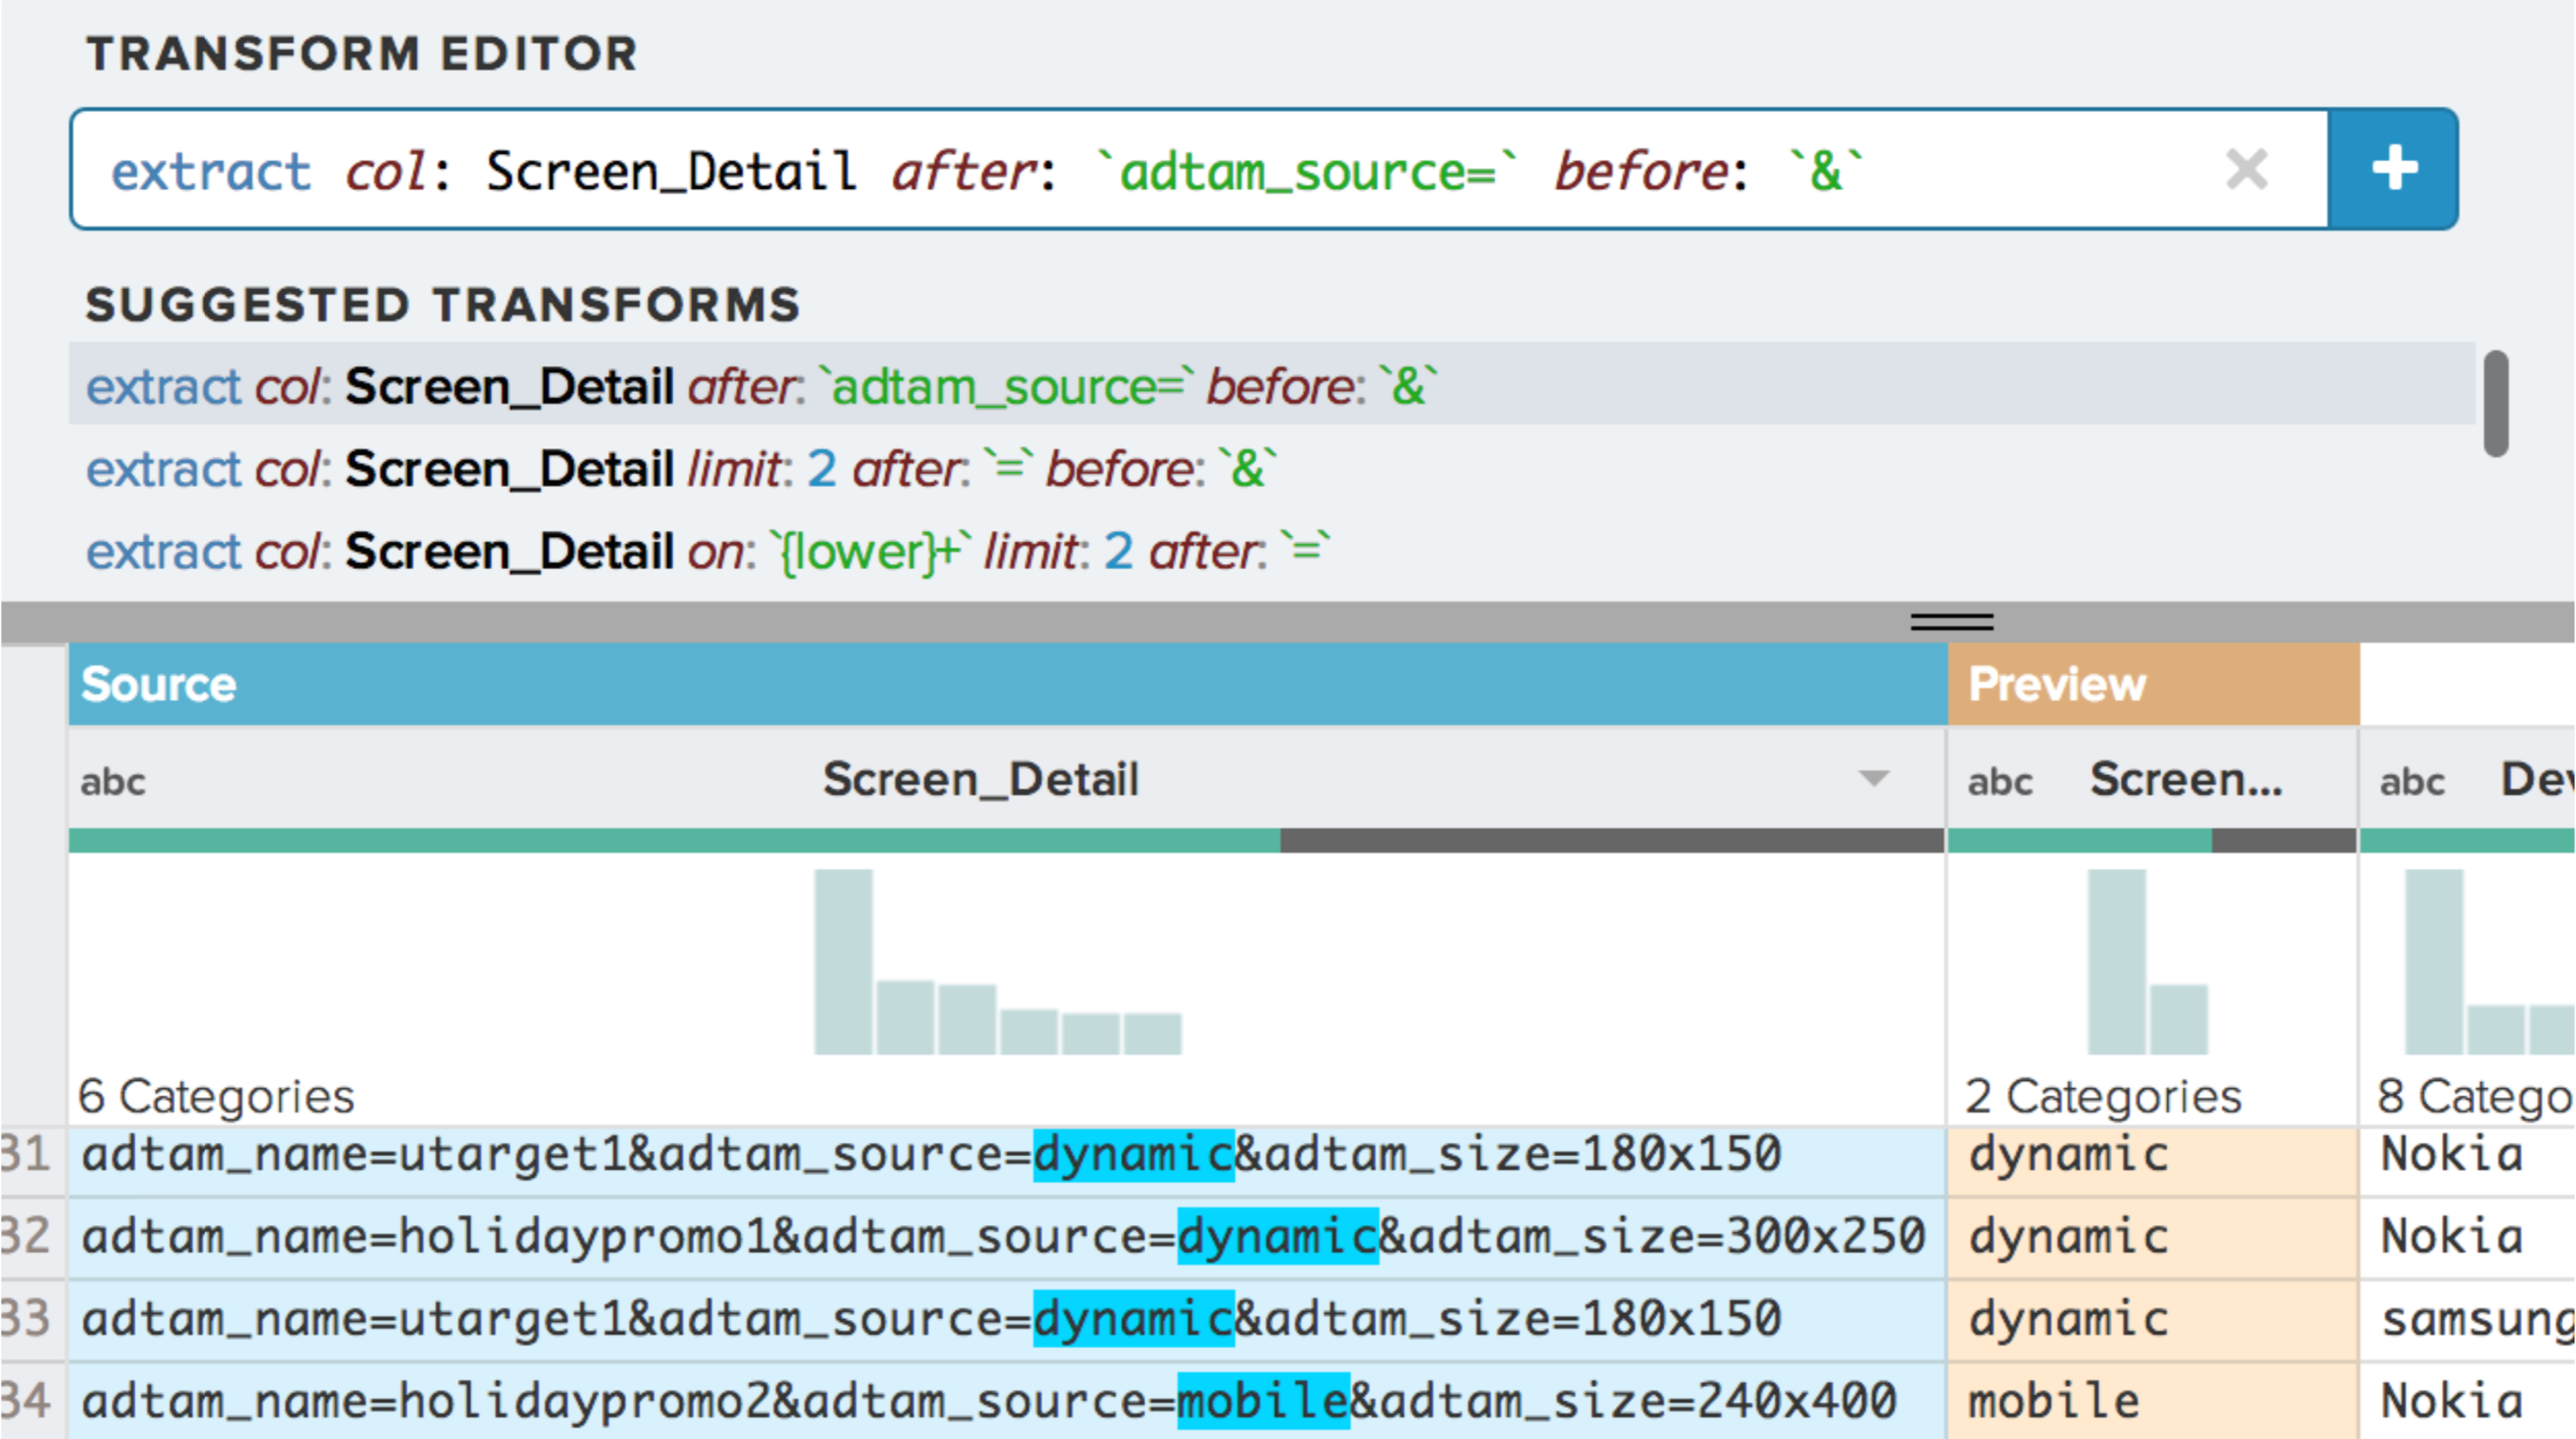
\includegraphics[width=0.4\textwidth]{figs/old_trifacta.png}
    \caption{An early version of Trifacta Wrangler, with explicit DSL editing.}
    \label{fig:trifacta_early}
\end{wrapfigure}
After founding Trifacta, we rebuilt the DSL and interface from the ground up. We maintained the predictive interaction approach, including visual transform previews. We incorporated more powerful means of transform customization. For example, predictions may be close to a user's intent but not a perfect match, requiring further refinement. Users also needed means to express custom calculation formulae. These requirements, combined with %limited engineering resources and 
a startup's zeal for agility, led to us to an early version that surfaced recommendations directly as DSL code statements, alongside a code editor for drafting or modifying statements (Figure~\ref{fig:trifacta_early}). This provided maximal expressiveness, but required learning the syntax of our Wrangle DSL. While valuable for trained users, user feedback indicated that this design imposed an unattractive learning curve for our target personas.

We also incorporated \emph{visual profiles}: automatically-generated summary visualizations that convey the shape and structure of the data. We added histograms to the column headers in the grid view, while also providing dedicated per-column views with statistical summaries and type-specific visualizations, such as maps for geospatial data and aggregate trends by month, week, day, \emph{etc.}{} for temporal data. Akin to interaction with table cells, interaction with visual profiles trigger transform suggestions, for example filtering to a selected data range.
\begin{wrapfigure}{R}{0.6\textwidth}
    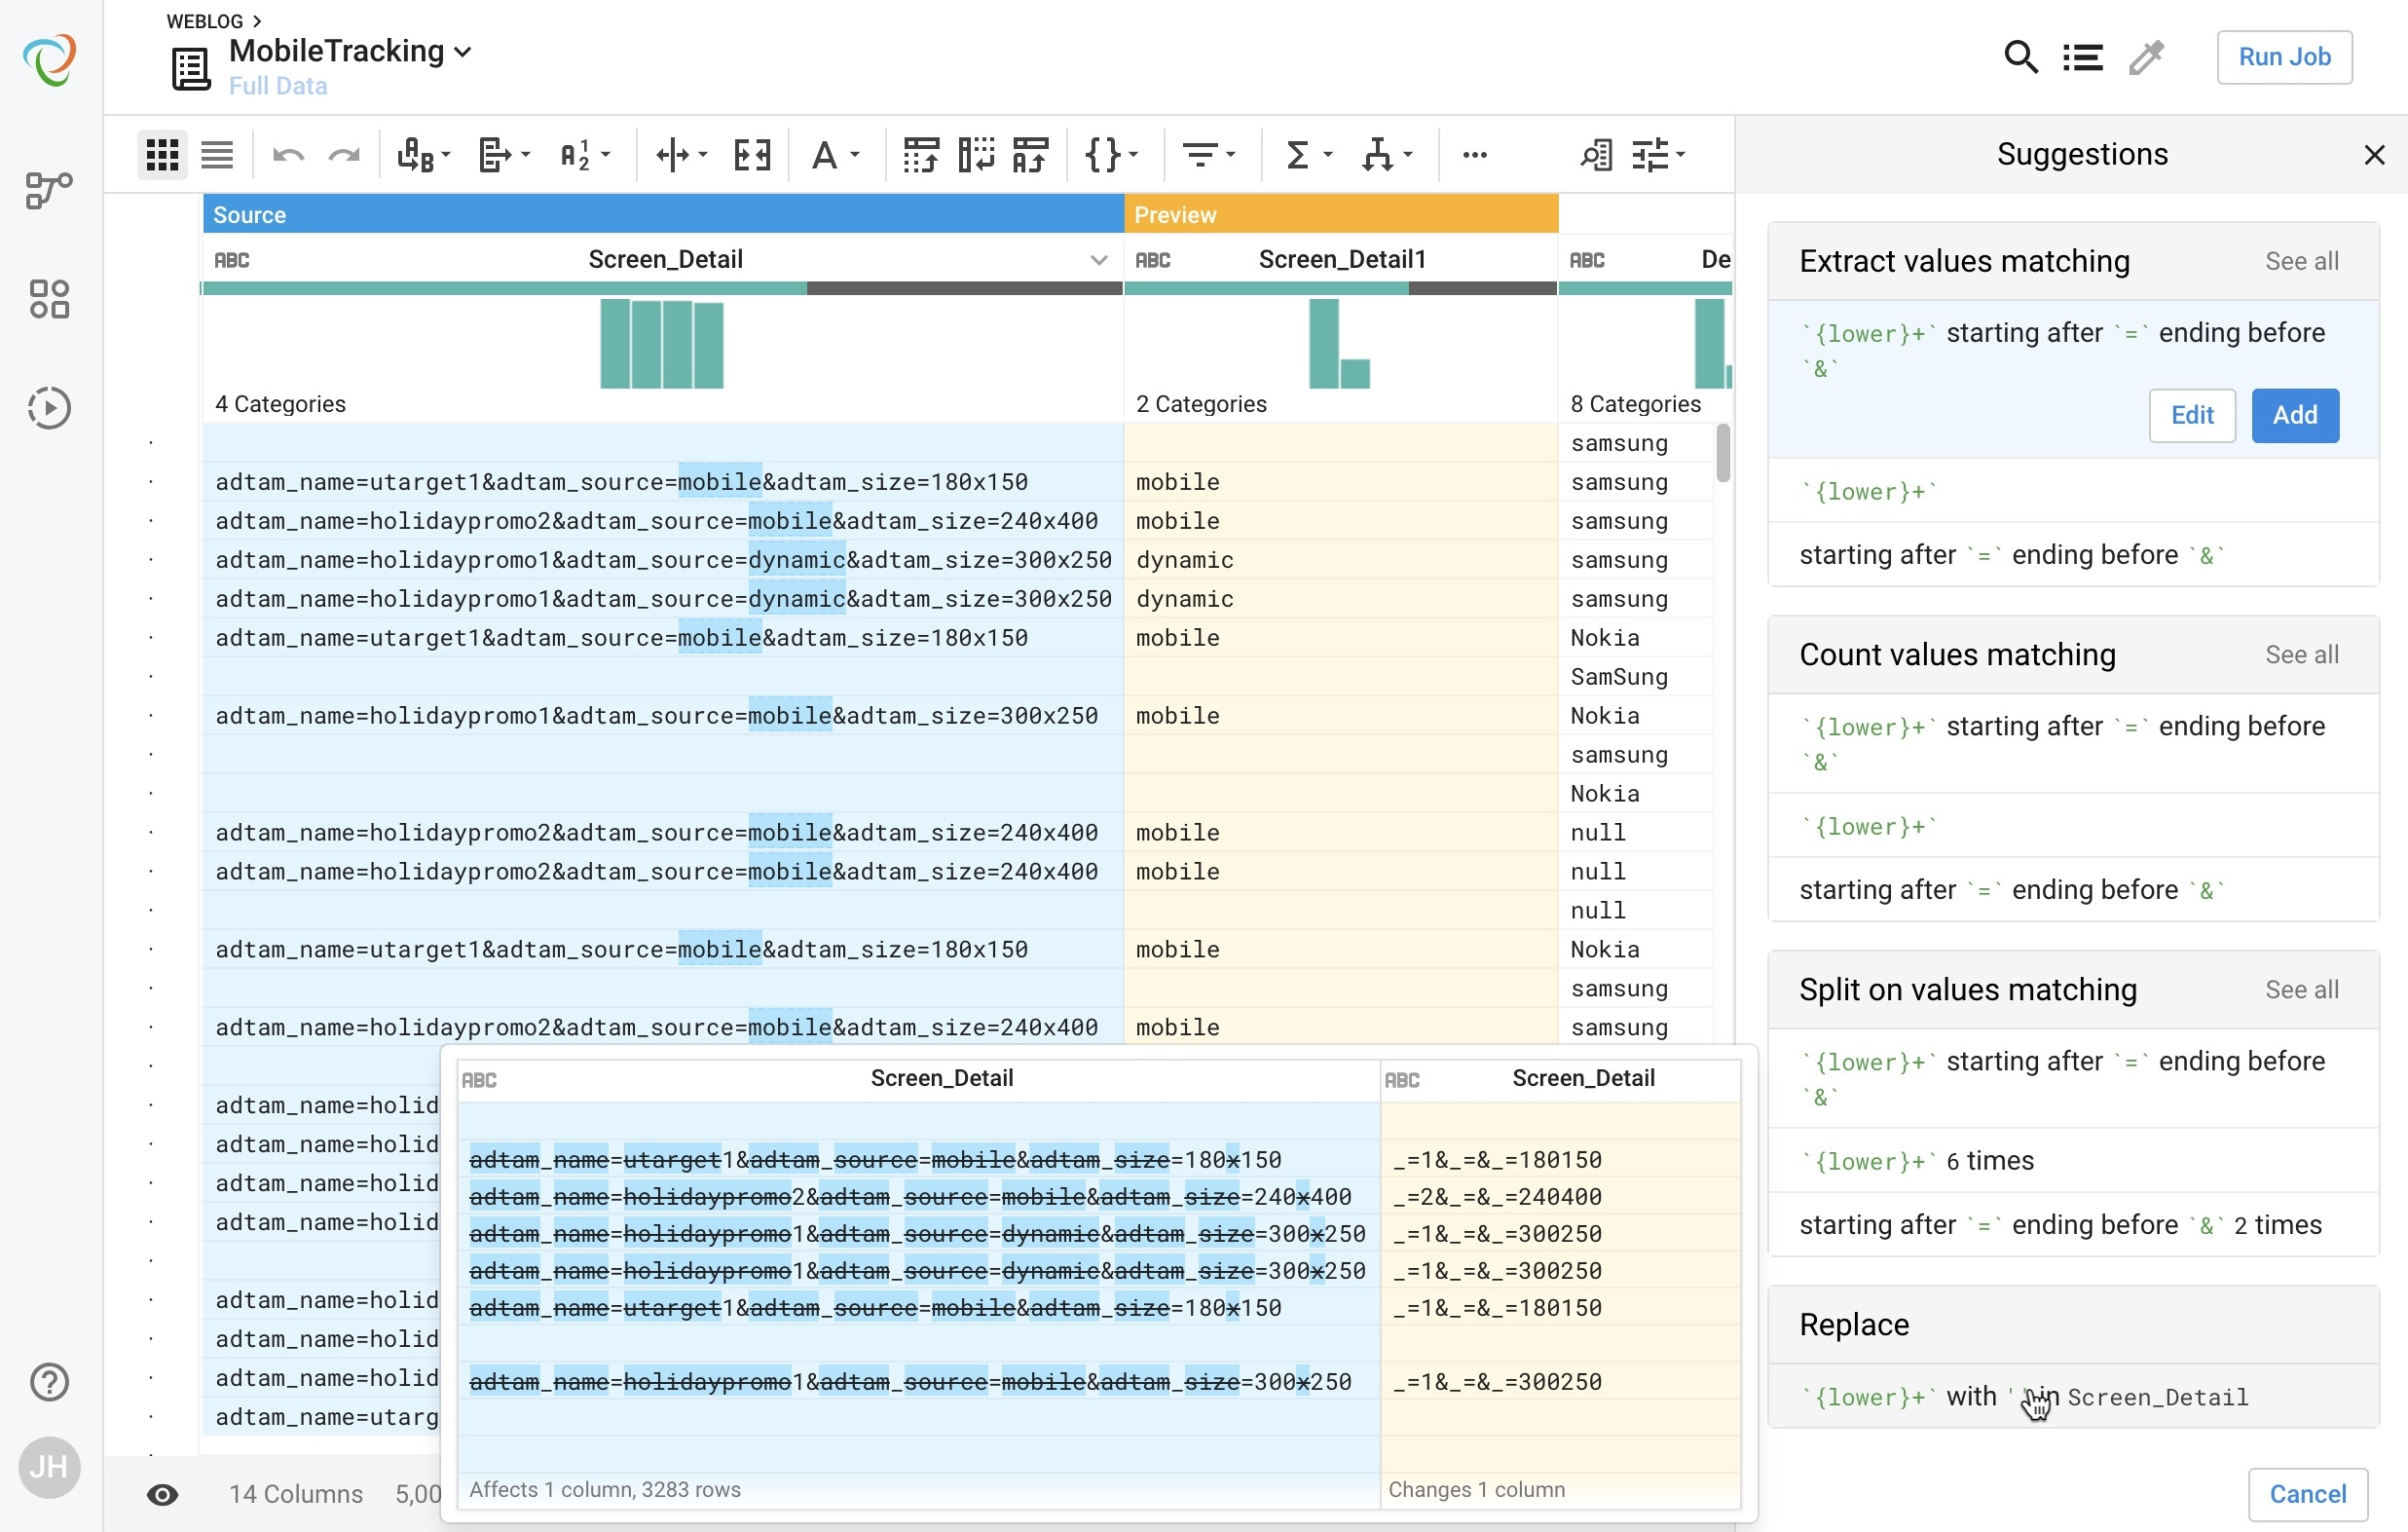
\includegraphics[width=0.6\textwidth] {figs/trifacta-cards.jpeg}%{figs/WorkflowBasics-ReplaceValues.png}
        \caption{Trifacta Wrangler with suggestion cards. The first suggestion highlighted in blue is previewed in the main grid. Hovering over an alternative suggestion (low in the list) yields a visual preview of its effects.}
        \label{fig:trifacta_cards}
\end{wrapfigure}

As both our product and personas evolved, we further elaborated the interface model with additional features. For example, we sought to improve users' ability to interpret transform suggestions through the inclusion of a navigable gallery of small visual summaries of suggested transformations. As shown in Figure~\ref{fig:trifacta_cards}, these \emph{cards} pair DSL code snippets with before \& after comparisons to complement our existing visual previews.

To help users create new transforms or refine suggested ones without writing textual code, we developed a transform \emph{builder}: a structured graphical editor for transformation authoring and modification. Builder scaffolds the transformation authoring process with input widgets for each transform parameter (Figure~\ref{fig:trifacta_builder}). Users can directly configure a transform without having to learn the syntax of the underlying DSL. Builder also provides \emph{in situ} help and documentation to further aid the process. The transform types and parameters in builder are isomorphic to those in Wrangle DSL, facilitating learning over time. Finally, we found that many users migrating from traditional tools like Excel wanted a menu bar to browse for functionality; choosing an item from Trifacta's menu bar populates the builder with suggested parameters. 
\begin{wrapfigure}{R}{0.6\textwidth}
       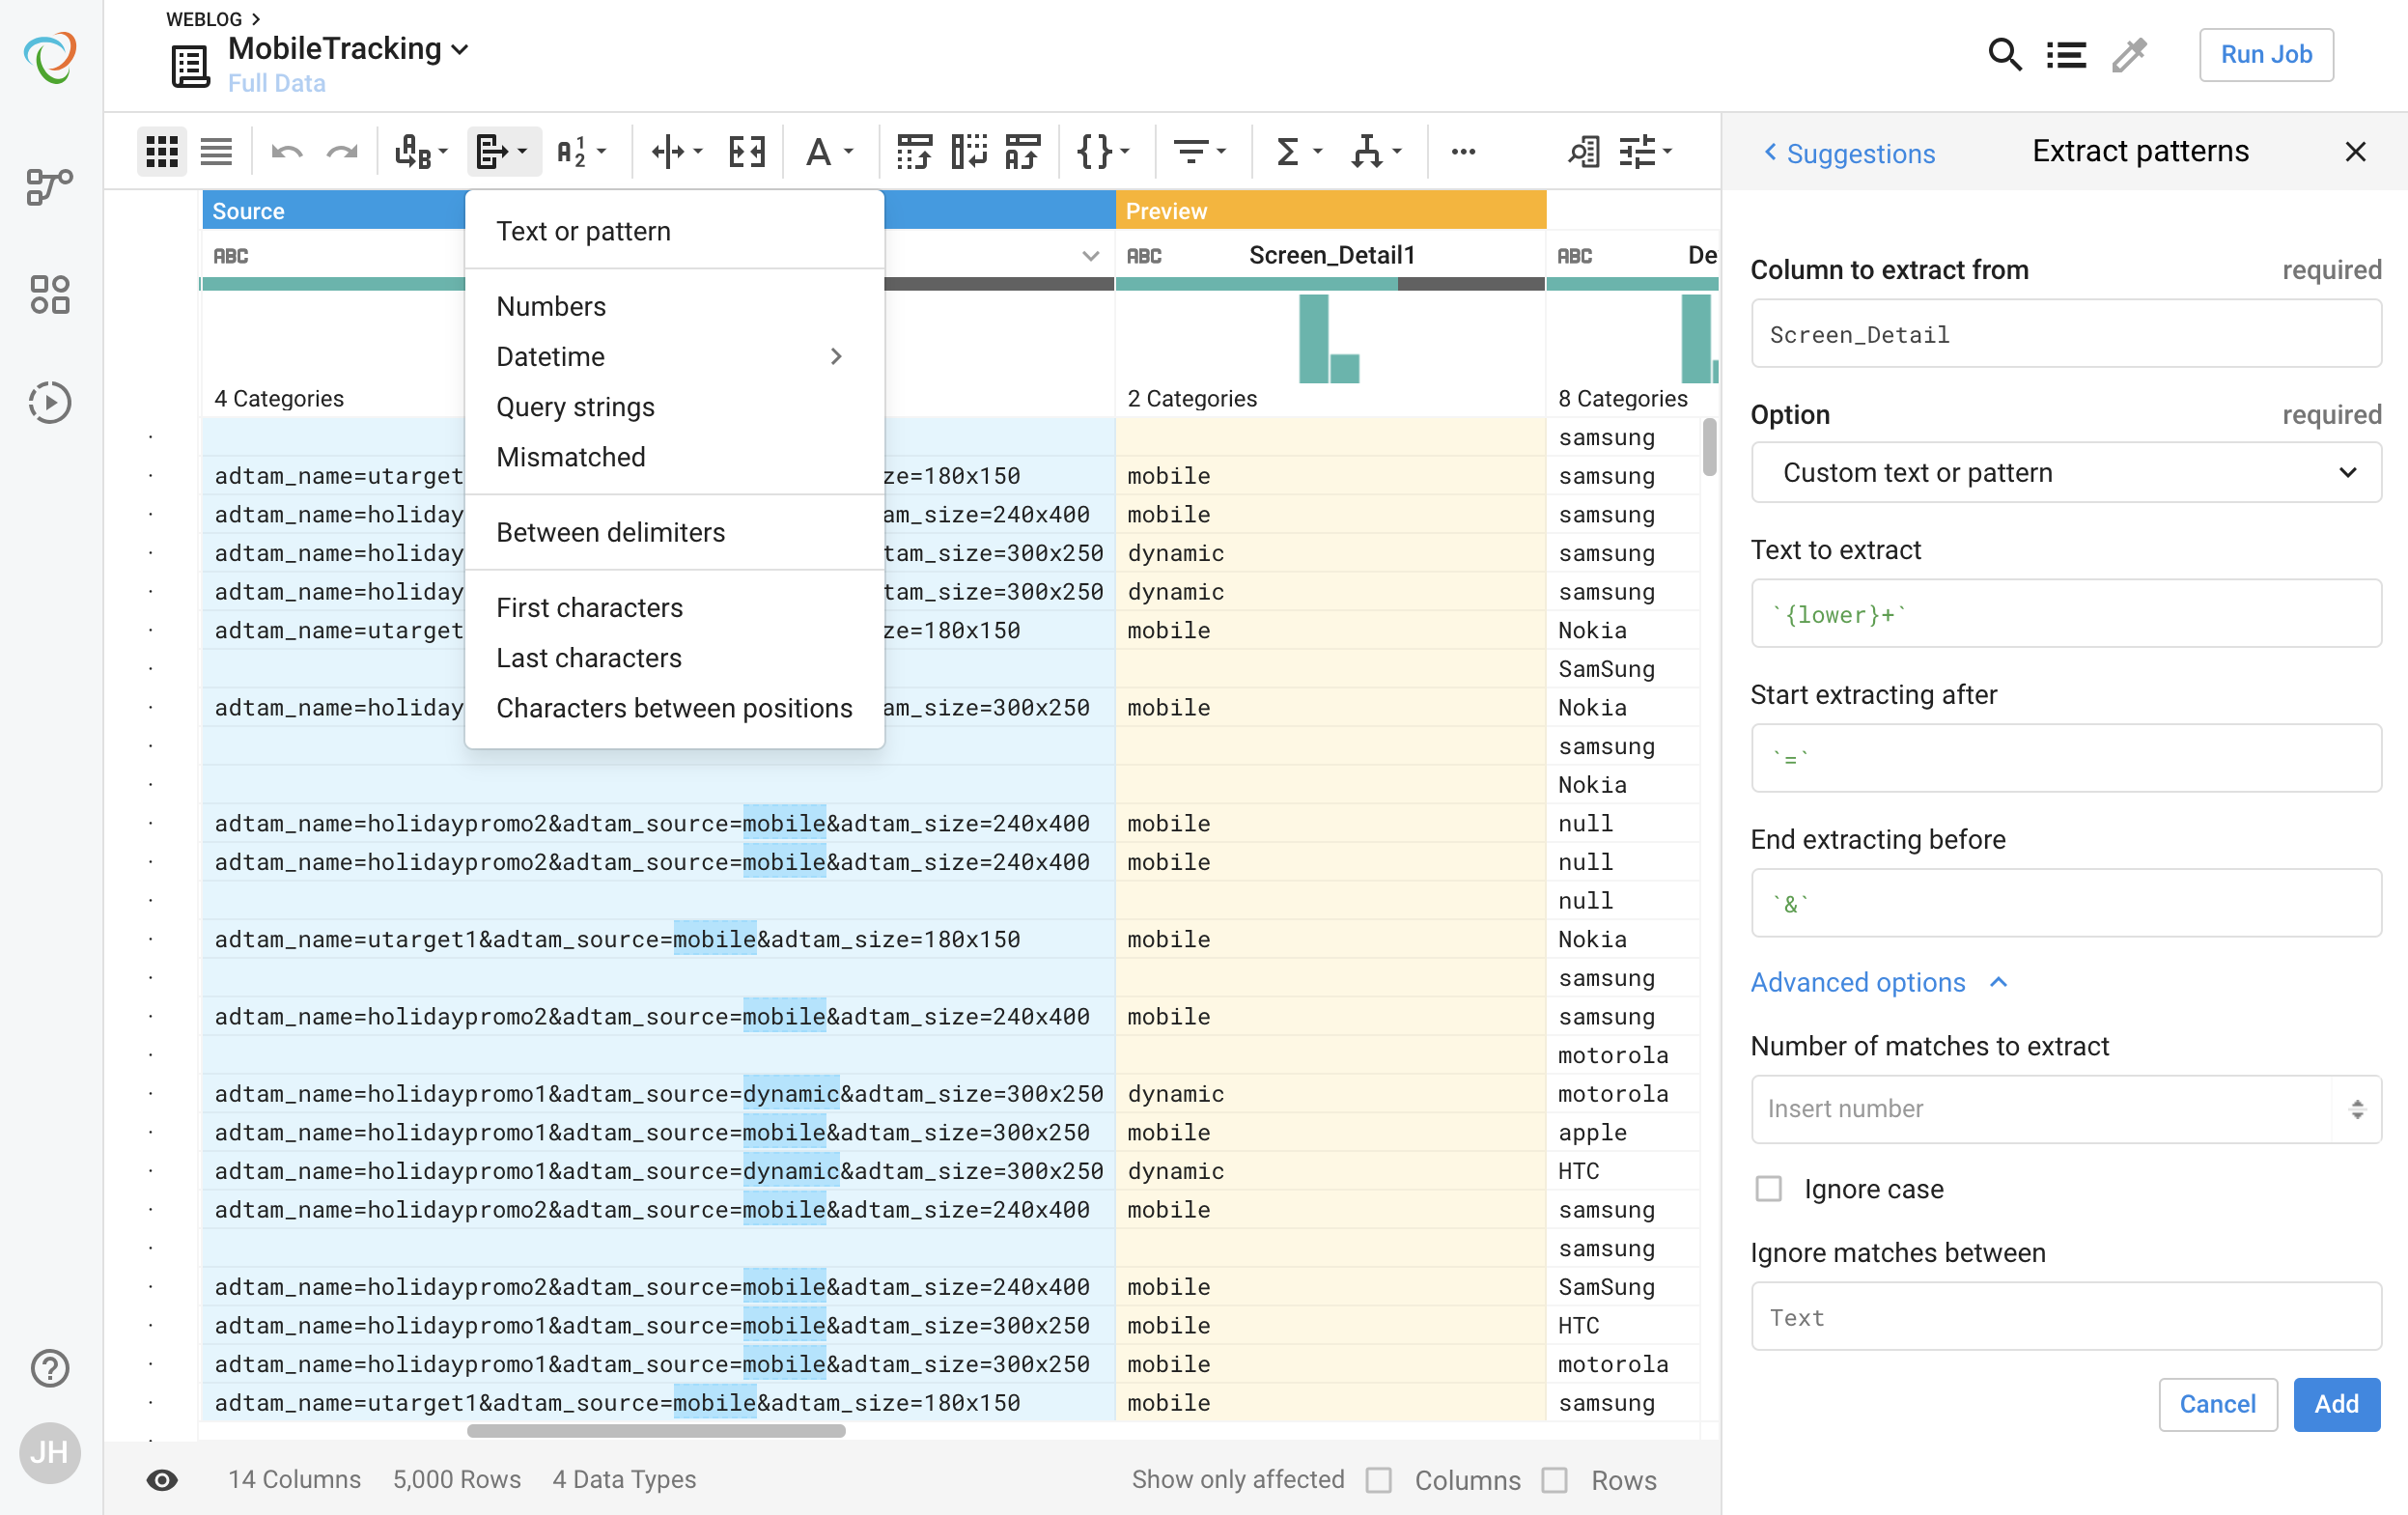
\includegraphics[width=0.6\textwidth]{figs/builder.png}
       \caption{Menus and builder for explicit transformation. Choosing a menu item opens and populates the builder interface on the right, which provides a structured graphical editor over the DSL code from Figure~\ref{fig:trifacta_early}.}
      \label{fig:trifacta_builder}
\end{wrapfigure}

\subsection{Architecture Evolution}
The original Potter's Wheel tool was built as a desktop application,
centered on a DSL of transforms that were surfaced as menu commands~\cite{raman2001potter}. (Many current data preparation tools are designed this way.)
Potter's Wheel was distinguished architecturally by a unique ability to allow instantaneous interaction on large datasets. It would begin scanning a file or table, and stream it immediately into an online reordering algorithm that bucketized the incoming data~\cite{raman1999online}. Sample rows would immediately appear in the user interface from buckets biased toward the current scrollbar position, giving the illusion of fluid scrolling over an unbounded table of data. Meanwhile, streaming anomaly detection algorithms could work in the background on the data while it was being scanned. 

Ten years later, the academic Wrangler prototype~\cite{wrangler} was implemented as a browser-based Javascript application. It accepted only very small datasets pasted into a text buffer, but focused on generating not only output data, but output~\emph{scripts} in one of a variety of external languages including Javascript, Python, SQL and MapReduce.  
This shift in primary focus from data manipulation to code generation was critical in the design of Trifacta.

When designing Trifacta's first version in 2012, we were interested in extending the reach of Wrangler beyond casual web use to a full range of challenging data-rich scenarios. Our goals included tackling a rich variety of data representations, from unstructured to semi-structured and relational data. We were also determined to address potentially unbounded volumes of data---not just generating ``big data'' code as a proof of concept, but working in a seamless and performant way in a big data ecosystem.

This led us to consider two deployment targets. The first was to host Trifacta Wrangler, this time as a scalable service embedded in public cloud infrastructure. The second choice was to deliver an on-premises solution that would integrate with the emerging ``big data'' stack. Architecturally, we believed that a design targeted to run as a service would also work well on premises, so we essentially designed for running as a service. As it happened, 2012 was far too early for most enterprise customers to bring serious data to the cloud, so we opted to deliver Trifacta as an on-premises ``big data'' solution first. However, when Google approached us four years later to deliver Trifacta as a service called Google Cloud Dataprep, we were architecturally in a good position to meet that challenge, and now we have offerings on all three public clouds.


\subsubsection{Trifacta Architecture}


The key goals of Trifacta's coarse-grained architecture were to scale from a single-user desktop up to the biggest SaaS deployments in the cloud, while preserving end-user simplicity and immediacy at every scale.

Trifacta was designed from the start as a three-tier solution, consisting of a Trifacta client built on browser technology (currently both Javascript and WebAssembly), a middle tier of soft-state Trifacta services, and a lower tier of commodity (non-Trifacta) services for persistence and big-data compute. The lower tier was designed to be pluggable with a variety of cloud-hosted or on-premises solutions including the Apache big data stack for on-premises deployment, and the native services of the popular public clouds. Key to this design was the focus going back to Potter's Wheel of having a DSL representation of user intent at the heart of the system, and---like Wrangler---an ability to cross-compile that DSL to multiple candidate execution services.

\begin{wrapfigure}{R}{0.45\textwidth}
    \centering
    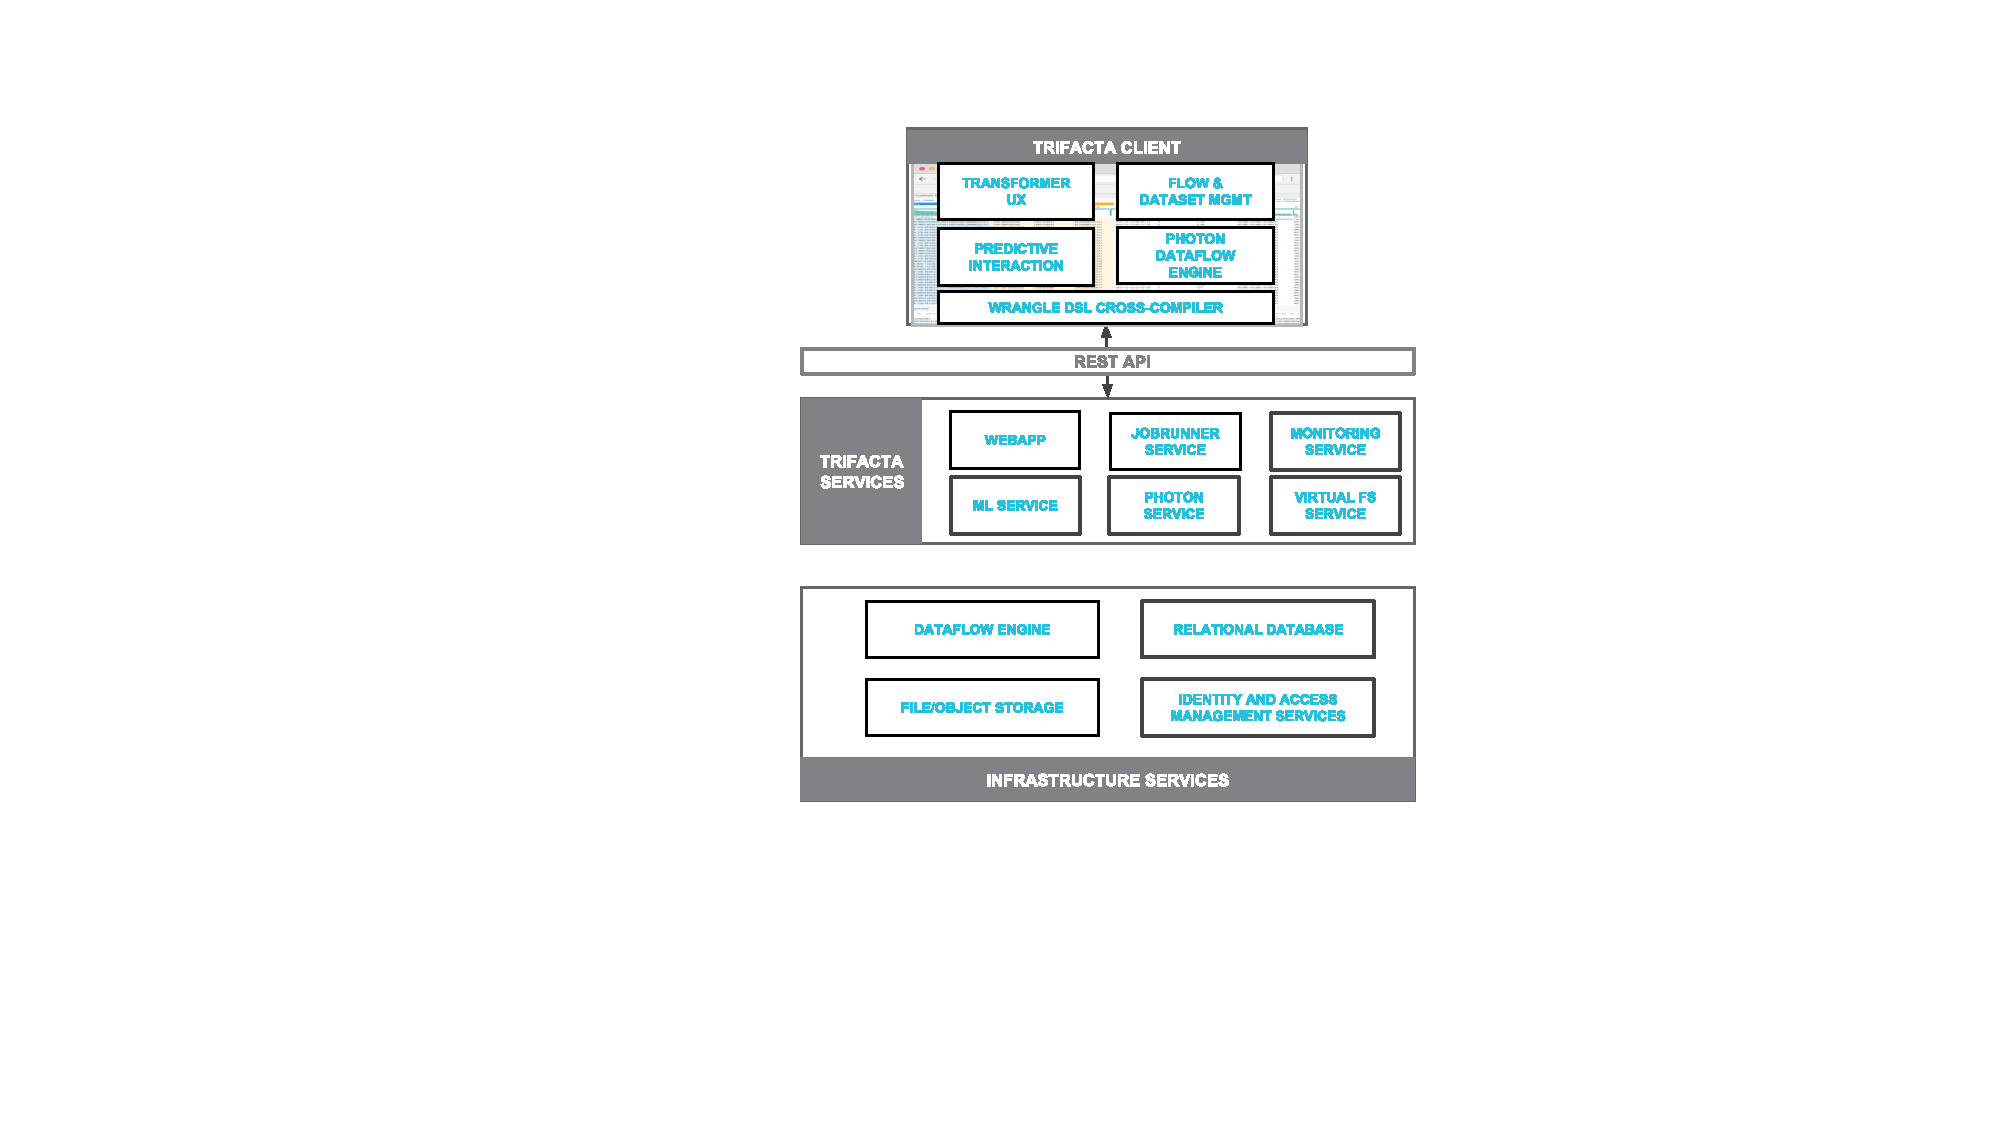
\includegraphics[width=0.45\textwidth]{figs/arch.pdf}
    \caption{Sketch of Trifacta Wrangler Enterprise.}
    \label{fig:my_label}
\end{wrapfigure}
The top (``client'') tier of Trifacta runs in a web browser, or in a desktop application using web components via the Chromium framework. The Trifacta client combines an intelligent Transformer user interface with a DSL cross-compiler---both written in Javascript---and also includes a C++-based in-memory query engine called Photon~\cite{photon} that is compiled to WebAssembly to run in the browser. The user interface includes many of Trifacta's characteristic visual profiling and ML-based predictive interaction~\cite{cidr-pi} model for transformation, as well as the ability to manage flows and external datasets from a wide variety of remote sources: filesystems, web-based storage, databases and so on. When a user identifies a dataset of interest, Trifacta's middle tier fetches the raw data and pushes it into the browser for initial visualization; if the dataset will not fit in browser memory, the middle tier pushes a sample of the data into the browser. As the user manipulates data in the Transformer interface, ``recipes'' (transformation scripts) are generated in Trifacta's DSL, ``Wrangle''. 
For every action in the Transformer interface, the recipe up to that point is compiled into a Photon query plan, executed by Photon on the browser-based data, and rendered on screen in a range of visualizations. This provides a rich, responsive direct-manipulation experience in the browser, and ensures that users can fluidly explore and transform their data without any backend processing. When the user chooses to run or schedule a job, the front-end cross-compiles their recipe to the backend execution framework of choice in their deployment---the list of targets has evolved over time as big data engines have waxed and waned in popularity, but current offerings at this date include hosted editions of Photon, Apache Spark, Google Dataflow, AWS Elastic MapReduce, and Azure HDInsight.



Trifacta's rich interface places significant demands on Photon in the browser: nearly every user gesture generates a multitude of transformation tasks (queries)---different tasks for each different suggestion to the user---which all need to be run through Photon at the speed of human interaction 
% (under 0.5~seconds~\cite{heer-latency}) 
to generate visual previews. This need for concurrent, responsive query processing is the primary reason we built our own in-memory query engine.
Some products for data transformation use backend technologies like Spark for their interactive processing. In designing Photon, we evaluated Spark to back each client, but found that Spark's performance was far too unpredictable---in startup, latency and especially memory pressure---to service our interactive user experience. Instead, Photon was inspired by a number of similar high-performance in-memory query engines including Hyper~\cite{kemper2011hyper} (now embedded similarly in Tableau) and Cloudera Impala~\cite{impala}. An overview of the Photon architecture is beyond the scope of this paper, but was presented in a conference talk viewable online~\cite{photon}.

Trifacta's middle tier is a set of soft-state services that power the frontend, and connect it to scalable data processing and storage. First, there is a web application that routes requests and controls the user interface's metadata, including browsing and storage of a registry of user Flows, Datasets, scheduled jobs, collaborations with other users, and so on. There is a jobrunner for running transformation jobs in big data engines in the lower tier, and a monitoring service to track those jobs throug their lifecycle. There is a ``virtual filesystem'' service for abstracting access to datasets from various storage systems, and a backend C++ Photon engine for running jobs that are too large to run in the browser, but small enough to run most quickly in memory on a single machine. Finally there is a machine learning (ML) service for serving predictions from a variety of models that power Trifacta's intelligent features. A non-exhaustive list of these ML features includes auto-detection of data types, recommendation of transformation steps, recommendations for join keys, synthesis of regular expressions from textual examples, and extraction/conversion of canonical patterns for variant data (e.g., for understanding a mixture of date formats, log records, addresses and so on, and optionally standardizing them.) 

The bottom tier of a Trifacta installation is not Trifacta code at all---it is a set of commodity infrastructure services that provide persistence and compute resources. These include a relational database for maintaining user metadata for the webapp, a scalable file system for unstructured dataset inputs and outputs, a dataflow execution service (query processor) and native services for identity and access management (e.g., Kerberos). 

Trifacta also offers a REST API for integrating with third-party services and applications: for example for publishing clean datasets to downstream analytics or charting tools, or for reading and writing metadata and job lineage to third party data catalogs. This API is critical for Trifacta to ``play nice'' with other pieces of the data stack, including infrastructure as well as downstream user-facing applications.

\subsubsection{Agile Exploration of Big Data: Sampling}
A key design imperative for Trifacta is to allow users to see and directly manipulate their data during transformation, which requires a responsive user interface. For very large datasets, the only way to get responsive interaction is to reduce the data to an efficient size---either via precomputation (summary structures like data cubes) or via subsetting the data (using indexes or random samples). Because the process of data wrangling transforms the dataset step-by-step, it is infeasible to assume precomputed structure like cubes or indexes are available on the full dataset---these structures would have to be rebuilt after every transform step! Instead, for data wrangling to both scale up and provide an immediate, responsive user experience, sampling is in some form is quite natural. Data preparation products that do not offer built-in sampling either (a) do not provide a responsive user experience, or (b) effectively force the user to do sampling by hand outside the product. Worse, when users do their own sampling in many products, they often are only able to get a transformed copy of their sample data---the wrangling work they author in the product is not transferrable to the larger dataset.

Potter's Wheel scaled fluidly via a unique sampling technique integrated into the UI. The design was innovative but not without problems: the sampling was a best-effort approach on streaming read, and had randomness guarantees that were hard to interpret statistically. The user experience was unpredictable as well, in terms of what data would actually be seen during scrolling: in particular, if a user saw a particular row at some scrollbar location, it was not guaranteed that said row would still be there if they scrolled away and scrolled back~\cite{raman2002partial}. 

Wrangler, by contrast, took a simple approach that put the burden  on the user. Because Wrangler could only consume as much data as the OS ``clipboard'' could cut-and-paste, users with big datasets had to downsample their data themselves. 
Importantly, though, Wrangler could still be useful for users with big data sets:
after the user transformed their sample dataset to their satisfaction, Wrangler (like Potter's Wheel before it) could output a reusable transformation script to transform the full dataset using a variety of programming languages (Javascript, Python, SQL, etc.) Hence while Wrangler itself did not scale, it provided a clear ``contract'' to the user about how it could and could not help with large data sets.

%% Trifacta
Trifacta was designed to preserve Wrangler's spirit of user clarity, but with significantly better scale and automation using an approach we call \emph{sample-to-scale}. The goals of sample-to-scale are to guarantee a responsive but rich visual experience, to put users in control of sampling in intuitive and low-friction ways, and to ensure that users' visual work is encoded in recipes that can be run at scale on unbounded amounts of data.  To get started quickly when opening a new dataset, Trifacta loads the ``head'' of the dataset into the browser by default, while in the background Trifacta's services are assembling a statistically robust simple random sample on the fly. The user is alerted when the random sample is available, and can switch between samples in the browser at any time. Because Trifacta user behaviors are captured in declarative recipes, the new sample can be run through the existing recipe and rendered in the browser immediately, to allow the user to see how their recipe to that point would work on a different sample. Trifacta also allows users to specify specific sampling methods including stratified sampling on particular columns, samples that ensure that certain values appear in their output, or samples that ensure that certain anomalies of interest are in evidence so they can be addressed. For UX consistency, Trifacta remembers the samples that users have worked with, and ensures that it is possible to go back to prior states of transformation history with the same samples that were originally seen. Finally, when users are satisfied with the properties of their transformed sample (or samples) they can run a full job, which executes the recipe over the entire datasets and produces both an output file and a data profile. 

\subsection{Deployments}
Trifacta's architecture allowed us to deploy it in multiple environments. There are three basic patterns. 

In an \textbf{on-premises} deployment, the lowest tier is the customer's existing installation of Hadoop and Spark from vendors like Cloudera and Hortonworks. Trifacta's middle tier is deployed on an ``edge node'' that sits alongside the Hadoop cluster, and provides metadata storage via a relational database. 

We also offer a similar \textbf{cloud tenant} deployment for customers whose data lives in the cloud. In this format, Trifacta's middle tier runs in Kubernetes-managed containers on behalf of the client, and native cloud services (database, dataflow, filesystem) replace the metadata database and the various functions of Hadoop.

Trifacta can also be deployed as \textbf{multitenant SaaS}, as we do for Google Cloud Dataprep. In this configuration, Trifacta's middle tier is run in an elastic environment of containers managed with Kubernetes. Jobs are compiled to run on elastic cloud dataflow services like Google Cloud Dataflow. Metadata is stored in a multitenant cloud database. We have seen users of this deployment
% of Trifacta exercise the scale of the architecture, 
routinely transform petabytes of data and consume thousands of compute hours. Yet they share the same agile experience in the browser enjoyed by smaller user cases thanks to the immediacy of photon and the philosophy of sample-to-scale.

To stay connected to our roots in the academic Wrangler prototype, we maintain a free photon-based edition of Trifacta Wrangler for use by the general public at \url{https://www.trifacta.com}. The global community of data wranglers provides us with front-line awareness of how the software can be improved over time.

\section{Conclusion}
After years of scattered research, Self-Service Data Preparation has emerged as a significant category in the data industry. It has a different technical focus than legacy data integration/ETL due to evolution in the users who wrangle data, the variety of data they face, and the data systems they favor. Usage at major enterprises demonstrates that new technologies improve processes for experienced users, and enable new classes of users to wrangle their own data. The area remains important for further innovation across Databases, AI, PL and HCI; we encourage our fellow researchers to further explore industry reports on the area~\cite{bloor, dresner, gartner-peer-insights, forrester-wave,gartner-marketguide-2017} as well as free offerings of data preparation solutions online to get a sense of issues in the field.



\itemsep=1pt 
\begin{small}
\begin{thebibliography}{10}

\bibitem{bloor}
{Bloor Research International}.
\newblock {Self-Service Data Preparation and Cataloguing}, 2016.
\newblock
  \url{https://www.bloorresearch.com/research/self-service-data-preparation-cataloguing/}
  accessed 05/14/2018.

\bibitem{cdc}
{Center for Disease Control}.
\newblock The anatomy of an {HIV} outbreak response in a rural community, 2015.
\newblock
  \url{https://blogs.cdc.gov/publichealthmatters/2015/06/the-anatomy-of-an-hiv-outbreak-response-in-a-} \url{rural-community/},
  accessed 5/11/2018.

\bibitem{chu2016data}
Xu~Chu, et al. %Ihab~F Ilyas, Sanjay Krishnan, and Jiannan Wang.
\newblock Data cleaning: Overview and emerging challenges.
\newblock In {\em Proceedings of the 2016 International Conference on
  Management of Data}, pages 2201--2206. ACM, 2016.

\bibitem{doan2012principles}
AnHai Doan, Alon Halevy, and Zachary Ives.
\newblock {\em Principles of data integration}.
\newblock Elsevier, 2012.

\bibitem{dresner}
{Dresner Advisory Services}.
\newblock {End User Data Preparation Study}, 2015.
\newblock
  \url{https://www.trifacta.com/gated-form/trifacta-earns-top-ranking-in-end-user-data-preparation-study/},
  accessed 05/14/2018.

\bibitem{personas}
Kim Flaherty.
\newblock Why personas fail, 2018.
\newblock \url{https://www.nngroup.com/articles/why-personas-fail/}, accessed
  5/11/2018.

\bibitem{galhardas2000ajax}
Helena Galhardas, et al. %Daniela Florescu, Dennis Shasha, and Eric Simon.
\newblock Ajax: an extensible data cleaning tool.
\newblock In {\em ACM Sigmod Record}, 29(2):590, ACM, 2000.

\bibitem{gartner-peer-insights}
{Gartner}.
\newblock {Peer Insights: Data Preparation}.
\newblock \url{https://www.gartner.com/reviews/market/data-preparation-} \url{tools},
  accessed 05/14/2018.

\bibitem{gulwani2011automating}
Sumit Gulwani.
\newblock Automating string processing in spreadsheets using input-output
  examples.
\newblock In {\em ACM SIGPLAN Notices}, volume~46, pages 317--330. ACM, 2011.

\bibitem{proactive-wrangler}
Philip~J. Guo, et al. %Sean Kandel, Joseph Hellerstein, and Jeffrey Heer.
\newblock Proactive wrangling: Mixed-initiative end-user programming of data
  transformation scripts.
\newblock In {\em Proc. ACM User Interface Software \& Technology (UIST)},
  2011.

\bibitem{cidr-pi}
Jeffrey Heer, Joseph Hellerstein, and Sean Kandel.
\newblock Predictive interaction for data transformation.
\newblock In {\em Proc. Conference on Innovative Data Systems Research (CIDR)},
  2015.

\bibitem{photon}
Joseph~M. Hellerstein and Seshadri Mahalingam.
\newblock {Architecting Immediacy---The Design of a High-Performance Portable
  Wrangling Engine}.
\newblock In {\em Strata Conference}, March~31, 2016.

\bibitem{hernandez2001clio}
Mauricio~A Hern{\'a}ndez, Ren{\'e}e~J Miller, and Laura~M Haas.
\newblock Clio: A semi-automatic tool for schema mapping.
\newblock {\em ACM SIGMOD Record}, 30(2):607, 2001.

\bibitem{ravi}
Ravi Hubbly, 2018.
\newblock \url{https://www.trifacta.com/partners/leidos/}, accessed 05/16/2018.

\bibitem{ilyas2015trends}
Ihab~F Ilyas and Xu~Chu.
\newblock Trends in cleaning relational data: Consistency and deduplication.
\newblock {\em Foundations and Trends{\textregistered} in Databases},
  5(4):281--393, 2015.

\bibitem{jin2017foofah}
Zhongjun Jin, et al. %Michael~R Anderson, Michael Cafarella, and HV~Jagadish.
\newblock Foofah: Transforming data by example.
\newblock In {\em Proceedings of the 2017 ACM International Conference on
  Management of Data}, pages 683--698. ACM, 2017.

\bibitem{kandel2011wrangler}
Sean Kandel, et al. %Andreas Paepcke, Joseph Hellerstein, and Jeffrey Heer.
\newblock Wrangler: Interactive visual specification of data transformation
  scripts.
\newblock In {\em Proceedings of the SIGCHI Conference on Human Factors in
  Computing Systems}, pages 3363--3372. ACM, 2011.

\bibitem{wrangler}
Sean Kandel, et al. % Andreas Paepcke, Joseph Hellerstein, and Jeffrey Heer.
\newblock Wrangler: Interactive visual specification of data transformation
  scripts.
\newblock In {\em Proc. ACM Human Factors in Computing Systems (CHI)}, 2011.

\bibitem{interviews}
Sean Kandel, et al. %Andreas Paepcke, Joseph Hellerstein, and Jeffrey Heer.
\newblock Enterprise data analysis and visualization: An interview study.
\newblock In {\em Proc. IEEE Visual Analytics Science \& Technology (VAST)},
  2012.

\bibitem{kemper2011hyper}
Alfons Kemper and Thomas Neumann.
\newblock Hyper: A hybrid oltp\&olap main memory database system based on
  virtual memory snapshots.
\newblock In {\em ICDE}, pages 195--206, 2011.

\bibitem{impala}
Marcel Kornacker and Justin Erickson.
\newblock Cloudera impala: Real time queries in apache hadoop, for real.
\newblock {\em Cloudera Engineering Blog}, October 2012.

\bibitem{leidos}
Leidos.
\newblock Deploying new tools for the fight against disease outbreaks, 2016.
\newblock
  \url{https://www.leidos.com/sites/default/files/responsive/Health/CAADS-Case-Study.pdf},
  accessed 5/11/2018.

\bibitem{forrester-wave}
Cinny Little, Gene Leganza, and Jun Lee.
\newblock {\em The Forrester Wave™: Data Preparation Tools, Q1 2017}.
\newblock Forrester, 2017.

\bibitem{mandelbaum2007pads}
Yitzhak Mandelbaum, et al.
\newblock PADS/ML: A functional data description language.
\newblock {\em ACM SIGPLAN Notices}, 42(1):77--83, ACM, 2007.

\bibitem{nyt-janitor}
Steve Lohr.
\newblock {For Big-Data Scientists, ‘Janitor Work’ Is Key Hurdle to
  Insights}.
\newblock {\em The New York Times}, August~17, 2014.

\bibitem{marcus2015crowdsourced}
Adam Marcus and Aditya Parameswaran.
\newblock Crowdsourced data management: Industry and academic perspectives.
\newblock {\em Foundations and Trends{\textregistered} in Databases},
  6(1-2):1--161, 2015.

\bibitem{novet-dataprep}
Jordan Novet.
\newblock {Google launches Cloud Dataprep, an embedded version of Trifacta}.
\newblock {\em VentureBeat}, March~9, 2017.

\bibitem{patil2012data}
DJ~Patil.
\newblock {\em Data Jujitsu}.
\newblock O'Reilly Media, Inc., 2012.

\bibitem{raman2001potter}
Vijayshankar Raman and Joseph~M. Hellerstein.
\newblock Potter's wheel: An interactive data cleaning system.
\newblock In {\em VLDB}, volume~1, pages 381--390, 2001.

\bibitem{raman2002partial}
Vijayshankar Raman and Joseph~M. Hellerstein.
\newblock Partial results for online query processing.
\newblock In {\em Proceedings of the 2002 ACM SIGMOD international conference
  on Management of data}, pages 275--286. ACM, 2002.

\bibitem{raman1999online}
Vijayshankar Raman, Bhaskaran Raman, and Joseph~M. Hellerstein.
\newblock Online dynamic reordering for interactive data processing.
\newblock In {\em VLDB}, volume~99, pages 709--720, 1999.

\bibitem{rattenbury2015data}
T~Rattenbury, et al.%JM~Hellerstein, J~Heer, and S~Kandel.
\newblock {\em Data Wrangling: Techniques and Concepts for Agile Analytics}.
\newblock O'Reilly, Sebastopol, CA, 2015.

\bibitem{nyt}
Megan Twohey.
\newblock {Mike Pence's} response to {H.I.V}. outbreak: Prayer, then a change
  of heart.
\newblock {\em The New York Times}, August~7, 2016.

\bibitem{datanami}
Alex Woodie.
\newblock Tracking the opioid-fueled outbreak with big data.
\newblock {\em Datanami}, December~15, 2016.

\bibitem{gartner-marketguide-2017}
Ehtisham Zaidi, Rita~L. Sallam, and Shubhangi Vashisth.
\newblock {\em Market Guide for Data Preparation}.
\newblock Gartner, December~14, 2017.
\end{thebibliography}
\end{small}

\end{document}
% 